\documentclass{beamer}
%
% Choose how your presentation looks.
%
% For more themes, color themes and font themes, see:
% http://deic.uab.es/~iblanes/beamer_gallery/index_by_theme.html
%
\mode<presentation>
{
  \usetheme{Warsaw}      % or try Darmstadt, Madrid, Warsaw, ...
  \usecolortheme{default} % or try albatross, beaver, crane, ...
  \usefonttheme{default}  % or try serif, structurebold, ...
  \setbeamertemplate{navigation symbols}{}
  \setbeamertemplate{caption}[numbered]
} 

\usepackage[english]{babel}
\usepackage[utf8x]{inputenc}
\usepackage{graphicx}
\usepackage[ELEC]{aaltologo}
%\usepackage{animate}
\usepackage{hyperref}

\title[ZigBee]{Alternative Network Architectures: ZigBee}
\author{Riku Lääkkölä \and Tero Marttila \and Tero Paloheimo}
\institute{Aalto ELEC}
\date{25.3.2014}
\logo{\AaltoLogoRandomSmall{0.3}}

\begin{document}

\begin{frame}
  	\titlepage
\end{frame}

% Uncomment these lines for an automatically generated outline.
%\begin{frame}{Outline}
%  \tableofcontents
%\end{frame}

\begin{frame}{ZigBee}
  \begin{itemize}
    \item ZigBee builds on top of IEEE 802.15 LR-WPAN
    \item Provides multi-hop/mesh networking
    \item Used for e.g. home automation, power meters, ...
    \item Applications with low data rates and low power consumption.
  \end{itemize}
  \begin{quotation}
  [...] individual devices must have a battery life of at least two years to pass ZigBee certification
  \end{quotation}
\end{frame}

\begin{frame}{IEEE 802.15}
  \begin{itemize}
  	\item IEEE 802.15.4
  	\item Low-Rate Wireless Personal Access Networks
	\item Defines Physical and Link layers
  	
    % ZigBee ISA100.11a WirelessHART.
  \end{itemize}
\end{frame}

\begin{frame}{IEEE 802.15 Physical Layer}
  \begin{itemize}
  	\item Provides low-bandwidth transmissions
  	\begin{itemize}
  		\item 868/915 MHz @ 20kbps and 2.4 GHz @ 250kbps
  	\end{itemize}
  	\item Optimized for cheap, low-power hardware
  	\begin{itemize}
    	\item Wakeup from sleep in 30ms (ZigBee)
  	\end{itemize}
  	\item Certification 
  \end{itemize}
  \begin{quotation}
  	An uncertified physical layer that malfunctions could cripple the battery lifespan of other devices on a ZigBee network.
  \end{quotation}
\end{frame}

\begin{frame}{ZigBee Physical Layer}
  \begin{figure}
  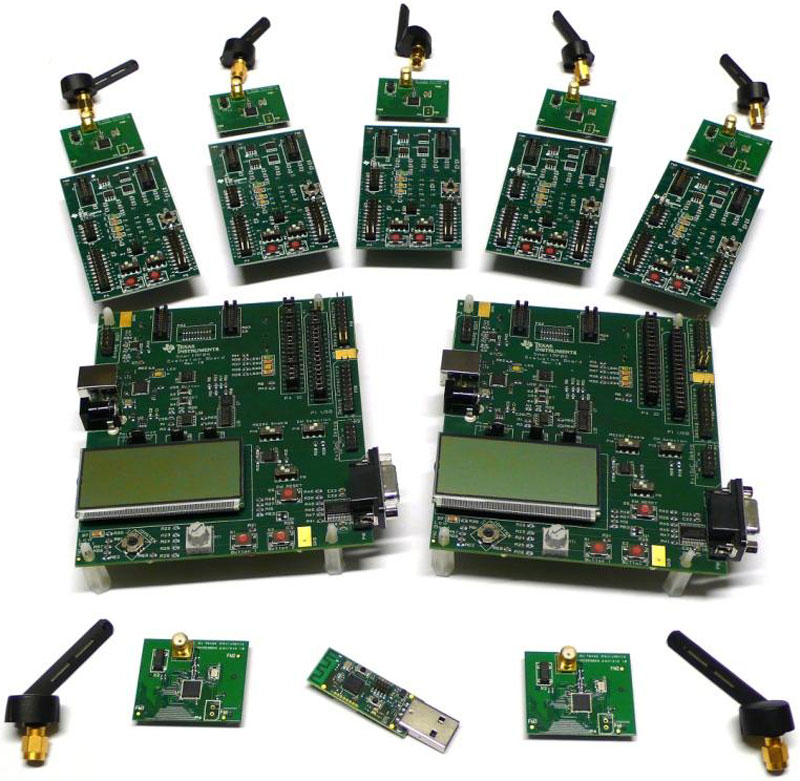
\includegraphics[width=0.6\textwidth]{ti_zigbee_devkit}
  \caption{Texas Instrument ZigBee prototyping boards.}
  \end{figure}
\end{frame}
    
\begin{frame}{IEEE 802.15 Link Layer}
  \begin{itemize}
    % CSMA, beacons.
    \item Full-function vs Reduced-function devices
	\begin{itemize}
  		\item Battery-powered devices wake up from sleep to transmit
  		\item Less power-constrained devices can receive continuously
  		\item Coordinated beacon intervals -> timed wakeup for receive
	\end{itemize}
	
  	%\item Addressing (?)
  	%\item Frame validation, time slot guarantees, node assocations.
  	\item Devices form point-to-point assocations
  	\begin{itemize}
  		\item Coordinator nodes
  		\item Relaying frames
  		\item Storing frames for sleeping nodes
  	\end{itemize}
  \end{itemize}
\end{frame}

\begin{frame}{ZigBee Network Layer}
  \begin{itemize}
  	\item Support for various network structures
  	\begin{itemize}
  		\item Star, Tree, Mesh
  	\end{itemize}
  	\item AODV routing (broadcast request -> unicast response)
  	\item Device types
  	\begin{itemize}
  		\item ZigBee Coordinator
  		\item ZigBee Router
  		\item ZigBee End Device
  	\end{itemize}
  \end{itemize}
  
  \begin{quotation}
	ZigBee turns 802.15.4 into a low power multi-hop mesh network
  \end{quotation}
\end{frame}

\begin{frame}{ZigBee Network Layer}
  \begin{figure}
  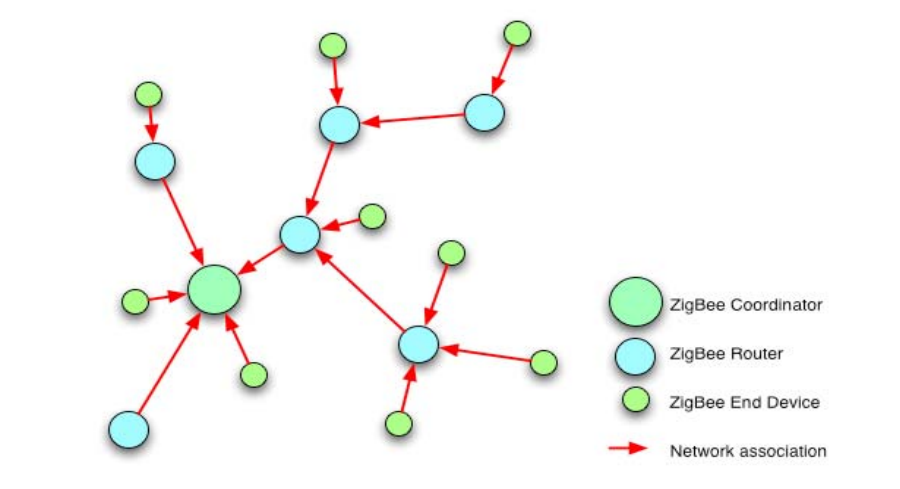
\includegraphics[width=\textwidth]{zbnetstructure.png}
  \caption{ZigBee network structure. Controllers and routers act as IEEE 802.15.4 FFDs and end devices as RFDs. Source \cite{zbslides}}
  \end{figure}
\end{frame}

\begin{frame}{ZigBee Application Layer}
  \begin{itemize}
  	\item ZigBee Device Object, Application Support Sublayer
  	\begin{itemize}
  		\item Form network topology
  		\item Service discovery
  		\item Security
  	\end{itemize}
  	\item Coordinator nodes maintain network state
  	\begin{itemize}
  		\item Service discovery
  		\item Security trust center
  	\end{itemize}
  	\item Application profiles
  	\begin{itemize}
  		\item Define application-specific protocols 
  	\end{itemize}
  \end{itemize}
\end{frame}

\begin{frame}{ZigBee Application Profiles}
  \begin{itemize}
  	\item ZigBee Home Automation
    \item ZigBee Smart Energy
    \item ZigBee Telecommunication Services
    \item ZigBee Health Care
    \item ZigBee RF4CE – Remote Control
    \item ZigBee RF4CE – Input Device
    \item ZigBee Light Link
    \item ZigBee IP
    \item ZigBee Building Automation
    \item ZigBee Gateway
    \item ZigBee Green Power
  \end{itemize}
\end{frame}

\begin{frame}{ZigBee Scale}
  \begin{itemize}
	\item Scales via use of ZigBee Routers
	\item Limited by global ZigBee Coordinator
  \end{itemize}
\end{frame}

\begin{frame}{References}
\begin{thebibliography}{9}
\bibitem{zbslides}
\url{https://docs.zigbee.org/zigbee-docs/dcn/06/docs-06-4513-00-00mg-zigbee-network-layer-technical-overview.pdf}
\end{thebibliography}
\end{frame}

\end{document}
